\chapter{Les lentilles}

\setcounter{section}{-1}
\section{Propagation dans les diélectriques (rappels)}
\begin{wrapfigure}[10]{l}{5.5cm}
	\vspace{-5mm}
	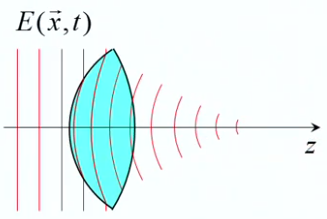
\includegraphics[scale=0.45]{ch3/image1.png}
	\captionof{figure}{ }
	\end{wrapfigure}	
Les lentilles étant faites en matériau diélectriques, il est intéressant de s'y attarder. Un diélectrique 
est un milieu constitué d'atomes qui conservent leurs électrons (à la différence des conducteurs). Si on 
place un atome dans un champ électrique, les charges positives constituant le noyau et les charges négatives
vont se déplacer dans des sens opposés sur 
un distance $x(t)$ (le champ électrique dépendant du temps). Ceci donne lieu à un dipôle oscillant.\\

\begin{wrapfigure}[6]{r}{9cm}
	\vspace{-5mm}
	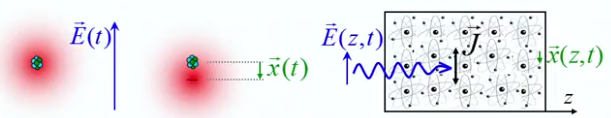
\includegraphics[scale=0.45]{ch3/image2.png}
	\captionof{figure}{ }
	\end{wrapfigure}
Dans un matériau diélectrique, on aura une vibration $\vec{x}(z,t)$ où $z$ est la coordonnée de propagation. 
Ceci donne lieu à des mouvements de charges dépendant de la position et du temps. Comme ces charges bougent, 
elles créent une densité de courant. On définit ainsi la \textit{densité de courant des charges liées}
\begin{equation}
\vec{J} = \eta_aq\dfrac{\partial \vec{x}}{\partial t}
\end{equation}
L'idée est d'aborder ça avec les équations de Maxwell
\begin{equation}
\left\{\begin{array}{ll}
\rot \vec{E} &= -\dfrac{\partial \vec{B}}{\partial t}\\
\rot \vec{B} &= \mu_0\vec{J} + \mu_0\epsilon_0\dfrac{\partial \vec{E}}{\partial t}
\end{array}\right.
\end{equation}
En prenant le rotationnel de la première équation
\begin{equation}
\rot(\rot\vec{E}) = -\dfrac{\partial \rot\vec{B}}{\partial t} = -\mu_0\dfrac{\partial \vec{J}}{\partial 
t} - \mu_0\epsilon_0\dfrac{\partial^2\vec{E}}{\partial t^2}
\end{equation}
La divergence étant nulle, le rotationnel du rotationnel donne $-\Delta$ ce qui donne, après simplification 
des signes négatifs
\begin{equation}
\Delta \vec{E} = \mu_0\dfrac{\partial\vec{J}}{\partial t}+\mu_0\epsilon_0\dfrac{\partial^2\vec{E}}{\partial 
t^2}
\end{equation}
En considérant le cas à une dimension en en faisant passer le second terme dans le membre de gauche tout en se rappelant que $\mu_0 \epsilon_0 = 1/c^2$ :
\begin{equation}
\dfrac{\partial^2\vec{E}}{\partial z^2} - \dfrac{1}{c^2}\dfrac{\partial^2\vec{E}}{\partial t^2} = \mu_0 
\dfrac{\partial\vec{J}}{\partial t}
\end{equation}
On retrouve exactement l'équation d'onde sans le terme de densité de courant de charges liées : le milieu 
introduit un terme en $\vec{J}$ un peu comme un terme de source. Avec l'expression de $\vec{J}$ :
\begin{equation}
\dfrac{\partial^2\vec{E}}{\partial z^2} - \dfrac{1}{c^2}\dfrac{\partial^2\vec{E}}{\partial t^2} = \mu_0 \eta_a 
q \dfrac{\partial^2\vec{x}}{\partial t^2}
\end{equation}

\begin{wrapfigure}[8]{l}{4cm}
	\vspace{-2mm}
	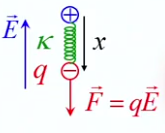
\includegraphics[scale=0.55]{ch3/image3.png}
	\captionof{figure}{ }
	\end{wrapfigure}
On voit apparaître l'accélération des charges, c'est elle et non le mouvement de translation qui génère des ondes. 
Notons que $\vec{x}$ est bien fonction du champ : comment $\vec{x}$ évolue en fonction du champ. Ceci 
permettra de "fermer" l'équation et ainsi de la résoudre. Pour se faire, adoptons le modèle des ressorts 
de Lorentz : le nuage électronique est lié aux noyaux comme une masse fixée à un ressort. Il est dès lors 
possible de lier ces deux variables. En faisant ceci, on réalise que l'on peut obtenir la solution suivante\footnote{
Les détails ne sont pas repris ici, c'est du rappel (cf. BA1).}
\begin{equation}
E(z,t) = E_\omega \cos[k(\omega)z-\omega t]
\end{equation}
La seule différence par rapport à la propagation dans le vide est que l'expression $k(\omega)$ est non 
triviale (dans le vide $k=\omega/c$). La résolution de l'équation d'onde (dérivée double par rapport à 
$z$) donne lieu à
\begin{equation}
k^2=\dfrac{\omega^2}{c^2}+\omega^2\mu_0\epsilon_0\chi(\omega) = \dfrac{\omega^2}{c^2}[1+\chi(\omega)]
\end{equation}
où $\chi(\omega)$ est la susceptibilité du milieu. Cette simple fonction contient l'information relative 
au movement des charges dans le diélectrique. En utilisant la \textit{perméabilité relative du mileu} 
$\epsilon_r = [1+\chi(\omega)]$, on peut écrire
\begin{equation}
k(\omega) = \dfrac{\omega}{c}\sqrt{\epsilon_r(\omega)} = \dfrac{\omega}{c} n(\omega)
\end{equation}
où $n(\omega) \equiv \sqrt{\epsilon_r(\omega)}$ est l'indice de réfraction. Il s'agit d'une fonction 
qui contient toute la dynamique des charges mises en mouvement par le champ électrique lui-même, elle 
reforme toute la complexité microscopique. On peut montrer que $c/n(\omega)$ est la \textit{vitesse de 
propagation (phase) de la lumière dans un diélectrique}\footnote{Pour le voir, mettre $k(\omega)$ en évidence 
dans la solution de l'équation d'onde $E(z,t)$.}
\begin{equation}
\hookrightarrow k(\omega) = \dfrac{\omega}{c}\sqrt{\epsilon_r(\omega)} = \dfrac{\omega}{c} n(\omega) = 
\dfrac{\omega}{v}
\end{equation}
L'indice de réfraction est le facteur de diminution de la vitesse de l'onde dans un diélectrique, 
l'indice de réfraction étant toujours plus grande que l'unité.
\begin{equation}
v = \frac{c}{n}
\end{equation}


Tout se base là-dessus. Étudions une lame de matériau diélectrique (verre) traversée par une onde 
plane monochromatique :
\begin{equation}
E(z,t) = E_\omega \cos[kz-\omega t]
\end{equation}
\newpage
\begin{wrapfigure}[8]{l}{6.4cm}
%	\vspace{-2mm}
	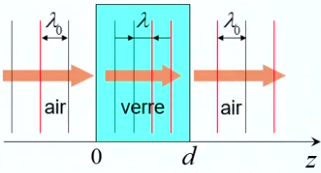
\includegraphics[scale=0.55]{ch3/image4.png}
	\captionof{figure}{ }
	\end{wrapfigure}
Avant de rentrer dans la lentille, l'onde plane se propage dans le vide : $k= k_0$ soit le 
nombre d'onde dans le vide et $\lambda_0 = \frac{2\pi}{k_0}$ la longueur d'onde dans le vide. Dans 
le milieu diélectrique, il ne faut \textbf{pas} reprendre $k_0$ mais $k = k_0n$ : la longueur 
d'onde sera plus petite, divisée par $n$, l'indice de réflexion est également le facteur de diminution 
de la longueur d'onde : $\lambda = \lambda_0/n$. \\

Interprétons ceci en nous basant sur la vitesse dans le diélectrique 
\begin{equation}
v = \frac{\omega}{n} = \frac{\omega}{k_0n} = \frac{c}{n}
\end{equation}

\begin{wrapfigure}[8]{r}{6.4cm}
	\vspace{-10mm}
	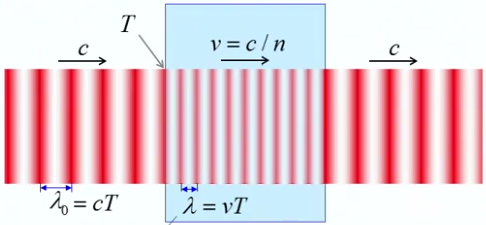
\includegraphics[scale=0.35]{ch3/image5.png}
	\captionof{figure}{Dans le vide $\lambda_0=cT$ et dans le verre $\lambda = vT$.}
	\end{wrapfigure}
La vitesse dans le diélectrique est moindre (les fronts d'ondes paraissent plus rapprochés), mais la 
période reste bien sûr inchangée. Le 
diélectrique cause un \textit{déphasage} : dans le diélectrique un front d'onde va "moins loin" que 
s'il était dans le vide (les fronts d'ondes seraient plus espacés), il y a donc distorsion de phase.\\


\begin{wrapfigure}[6]{l}{4.4cm}
	\vspace{-5mm}
	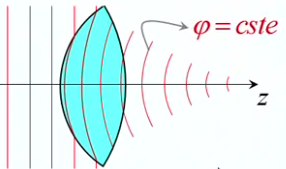
\includegraphics[scale=0.35]{ch3/image6.png}
	\captionof{figure}{ }
	\end{wrapfigure}
Une lentille c'est une lame à épaisseur variable causant un retard de phase variable (plus l'épaisseur 
de verre traversée est grande, plus cet effet de déphasage sera important). Les lieux de points de phases 
constantes, les fronts d'ondes, seront des surfaces à priori courbes.\\

Comme nous nous intéressons à la phase, aux fronts d'onde, regardons le phaseur
\begin{equation}
E(z,t) = E_\omega e^{ikz}e^{-i\omega t}
\end{equation}
La phase accumulée sur l'épaisseur $d$ lors de la traversée du diélectrique sera forcément $\varphi = kd = nk_0d$. 
Sans la lame de verre 
$\varphi = k_0d$. Le \textit{retard de phase (déphasage)} est obtenu en comparant la phase accumulée 
dans le verre avec celle dans le vide pour la même longueur traversée c'est à dire $d$
\begin{equation}
\Delta\varphi = k_0d(n-1)
\end{equation}
\textbf{Remarque} : un retard de phase est une phase qui évolue plus vite dans le diélectrique, mais 
il faut se souvenir que pour une distance donnée on a une "plus grande densité de fronts d'onde". Phase 
qui évolue rapidement veut dire retard de phase.\\


\newpage
\section{Fonction de transfert d'une lentille "mince"}
Le terme \textit{mince} a été introduit pour faire plusieurs approximation, on verra ça plus tard ! Le 
but de la fonction de transfert est de connaître le champ transmis par un simple produit avec le champ 
incident.
\begin{equation}
E_t(\vec{x}) = T(x,y)\times E_i(\vec{x})
\end{equation}

	\subsection{Lentilles à surfaces sphériques}
	\begin{wrapfigure}[7]{l}{4.4cm}
	\vspace{-5mm}
	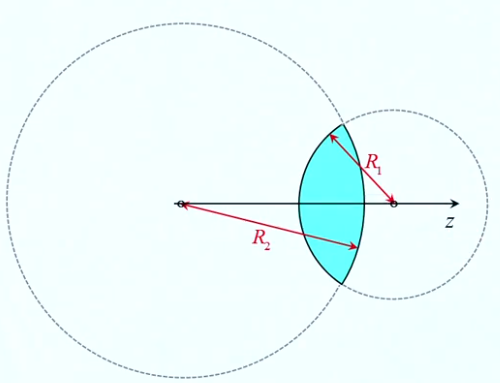
\includegraphics[scale=0.2]{ch3/image7.png}
	\captionof{figure}{ }
	\end{wrapfigure}
	L'idée d'une telle surface est que la surface est constituée de "morceau de surface de sphère", 
	la lentille peut être vue comme l'intersection de deux sphères. On nomme l'axe $z$ 
	l'\textit{axe optique} (axe reliant le centre des deux sphères) de la lentille (voir ci-contre). 
	L'épaisseur est variable en fonction de la position dans le plan transverse : son épaisseur 
	maximale est nommée $\Delta_0$.\\
	
	\begin{wrapfigure}[9]{r}{4.4cm}
	\vspace{-5mm}
	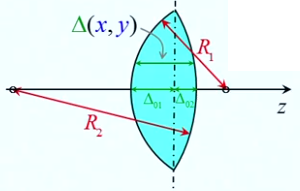
\includegraphics[scale=0.4]{ch3/image8.png}
	\captionof{figure}{ }
	\end{wrapfigure}
	Pour l'analyse, décomposons la lentille en deux demie-lentilles de rayons $R_1$ et $R_2$ respectivement
	: $\Delta_0 = \Delta_{01}+\Delta_{02}$. Ceci est 
	pour la hauteur maximale, mais on peut faire de même pour toute épaisseur
	\begin{equation}
	\Delta (x,y) = \Delta_1(x,y) + \Delta_2(x,y)
	\end{equation}
	Commençons par décrire la fonction $\Delta_1(x,y)$. Considérons un point du plan transverse $(x,y)$. 
	On se situe à $R_1$ du centre de courbure, que vaut cette épaisseur ? Faisons un peu de géométrie. 
	La distance de l'axe optique vaut $\sqrt{x^2+y^2}$ et celle depuis le centre de courbure vaut 
	$\sqrt{R_1^2-x^2-y^2}$ (par Pythagore). La distance entre l'extérieur de la lentille et la 
	coordonnée en $z$ de $(x,y)$ vaut $R_1-\sqrt{R_1^2-x^2-y^2}$. Pour exprimer $\Delta_1$, il suffit 
	de retirer à $\Delta_{01}$ cette distance que nous venons de calculer
	\begin{equation}
	\Delta_1(x,y) = \Delta_{01}-\left[ R_1-\sqrt{R_1^2-x^2-y^2}\right]
	\end{equation}
	De façon similaire, on trouve
	\begin{equation}
	\Delta_1(x,y) = \Delta_{02}-\left[ R_2-\sqrt{R_2^2-x^2-y^2}\right]	
	\end{equation}

	\begin{wrapfigure}[9]{l}{6.4cm}
	\vspace{-5mm}
	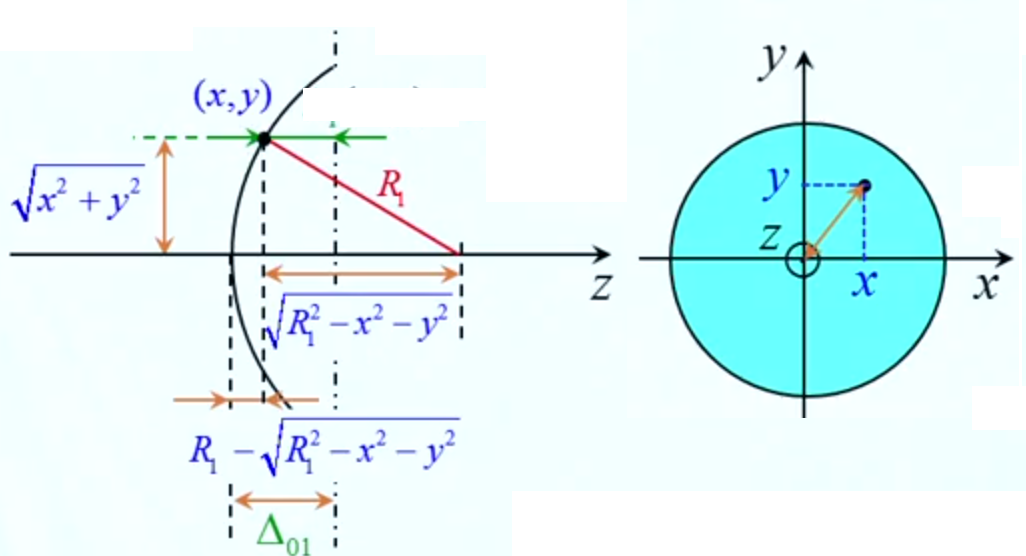
\includegraphics[scale=0.18]{ch3/image9.png}
	\captionof{figure}{ }
	\end{wrapfigure}	
	Comme nous l'avons précisé, nous allons considérer des lentilles \textit{minces} : fondamental 
	pour simplifier ces expressions. Il s'agit d'une lentille dont les rayons de courbures sont 
	très importants. Une lentille est mince lorsque sa distance transverse (taille de la lentille) 
	est petite par rapports aux rayons de courbures de ses surfaces 
	\begin{equation}
	\text{Lentilles "minces"} \qquad\Longrightarrow\qquad x^2+y^2 \ll R_1^2,R_2^2
	\end{equation}
	Il est dès lors possible d'utiliser l'approximation paraxiale/parabolique 
	\begin{equation}
	\Delta_1(x,y) = \Delta_{01}-\left[R_1-R_1\sqrt{1-\dfrac{x^2+y^2}{R_1^2}}\right] \approx \Delta_{01} -
	\left[R_1-R_1\left(1-\dfrac{x^2+y^2}{2R_1^2}\right)\right]
	\end{equation}
	Par calcul, on obtient
	\begin{equation}
	\begin{array}{ll}
	\Delta_1(x,y) &= \Delta_{01} - \dfrac{x^2+y^2}{2R_1}\\
	\Delta_2(x,y) &= \Delta_{02} - \dfrac{x^2+y^2}{2R_2}
	\end{array}
	\end{equation}
	La fonction $\Delta(x,y)$ est donnée en faisant la somme des deux termes
	\begin{equation}
	\Delta(x,y) = \Delta_0-\dfrac{x^2+y^2}{2}\left(\frac{1}{R_1}+\frac{1}{R_2}\right)
	\end{equation}
	
		\begin{wrapfigure}[9]{l}{6.4cm}
	\vspace{-5mm}
	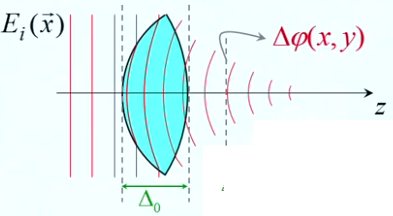
\includegraphics[scale=0.45]{ch3/image10.png}
	\captionof{figure}{ }
	\end{wrapfigure}	
	Cette expression permet d'étudier la fonction de transfert d'une lentille mince. Une lentille 
	propage des déphasages variables $\Delta \varphi(x,y)$. Afin de rester précis (la longueur d'onde 
	de la lumière étant petite, il vaut mieux%Qué ?)
	, on va étudier les déphasages dans un plan $z$ précis : 
	le profil de phase $\Delta\varphi(x,y)$ sera donné pour un plan bien précis. On définit alors le plan 
	d'entrée (tangeant à la première surface) et de sortie (tangent à la seconde). 
	
	\subsection{Lentilles "minces"}
	La fonction de transfert relie la champ incident aux champs transmis dans ce second plan. Ces deux 
	plans sont séparés de $\Delta_0 \ll R_1,R_2$. Nous allons faire l'approximation que ces deux plans 
	sont tellement rapprochés que l'on peut négliger la diffraction. Montrons le 
	\begin{equation}
	a(x,y;z) = \iint A(\rho,\sigma) e^{i\rho x}e^{i\sigma y} e^{i\sqrt{k^2-\rho^2-\sigma^2}z}\ d\rho d\sigma
	\end{equation}
	Dans le contexte de Fresnel (approximation paraxiale)
	\begin{equation}
	a(x,y;z) = \iint_{-\infty}^\infty A(\rho,\sigma)e^{i\rho x}e^{i\sigma y} e^{i\frac{\rho^2}{2k}z
	-i\frac{\sigma^2}{2k}z}\ d\rho d\sigma\ e^{ikz}
	\end{equation}
	Si on supprime les deux premières exponentielles de $z$ (le propagateur du spectre), on supprime 
	la diffraction
	\begin{equation}
	a(x,y;z) = \iint_{-\infty}^\infty A(\rho,\sigma)e^{i\rho x}e^{i\sigma y}\ d\rho d\sigma\ e^{ikz}
	\end{equation}
	Ceci est valable si $\max\rho$ est tel que puisque $\max z = \Delta_0$
	\begin{equation}
	\frac{\rho^2}{2k}\Delta_0 \ll 1
	\end{equation}
	Admettons-le pour le moment, on y reviendra. On a alors
	\begin{equation}
	a(x,y;z) = a(x,y;0)e^{ikz} = |a(x,y;0)|e^{i\varphi(x,y)}e^{ikz}
	\label{eq:amod}
	\end{equation}
	On retrouve un champ qui pris en module sera inchangé (le champ en $z$ sera le même que en 0). Le 
	propagateur a été réduit à son expression minimale : à une distance $z$, j'accumule une phase $kz$ quel 
	que soit le point du plan transverse dans lequel on se trouve. Cela correspond à une translation des 
	fronts d'onde comme illustré ci-dessous.
	
	\newpage

	\begin{wrapfigure}[8]{l}{6.4cm}
	\vspace{-3mm}
	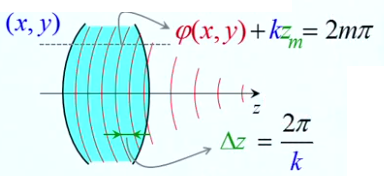
\includegraphics[scale=0.45]{ch3/image11.png}
	\captionof{figure}{ }
	\end{wrapfigure}		
	Regardons le lieu des points de phase constantes (de constante valant $2n\pi$)(def. front d'onde).
	Pour des valeurs de $x$ et $y$ fixé $\varphi(x,y) = c^{te}$ et on peut considérer que 
	l'équation ci-dessous, pour $x$ et $y$ donnés, donne les position en $z$ ou on trouve les 
	fronts d'onde.
	\begin{equation}
	\varphi(x,y) + kz_m = 2m\pi
	\end{equation}

	\begin{wrapfigure}[8]{r}{3.4cm}
	\vspace{-5mm}
	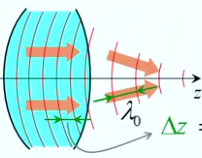
\includegraphics[scale=0.45]{ch3/image12.png}
	\captionof{figure}{ }
	\end{wrapfigure}				
	L'écart entre deux front d'onde est le même partout et vaut $\Delta z = 2\pi/k=\lambda$, la longueur d'onde et 
	ce peu importe où l'on se situe. Ce n'est "normal" que si on supprime la diffraction. Il faut remarquer 
	que le $\Delta z$ est pris parallèlement à l'axe $z$ alors que l'on considère la longueur d'onde 
	perpendiculairement au front d'onde, les deux situations sont différentes. Dans la lentille, on translate (rien 	    ne change entre 0 et $z$, pas de diffraction), alors que dans l'air le rayon de courbure devient de plus en plus petit (il y a en quelque sorte diffraction).\\

	Supposons que la variation du champ transverse incident se fait à une longueur caractéristique $\Delta l$. 
	On peut voir la lentille comme une fonction "fenêtre", limitant la taille du champ. C'est ce $\Delta l$ qui 
	va donner la valeur de $\rho$ pour étudier l'approximation. Pour se faire, regardons $A(\rho)$ la 
	transformée de Fourier de la fonction fenêtre, un sinc. La valeur maximal de $\rho$ vaut $\approx 2\pi/
	\Delta l$. Dans notre approximation
	\begin{equation}
	\frac{\rho^2}{2k}\Delta_0 \ll 1\qquad \Leftrightarrow\qquad \dfrac{4\pi^2\Delta_0}{2k\Delta l^2}\ll 1
	\end{equation}
	avec $k=2\pi/\lambda$ :
	\begin{equation}
	\Delta_0 \ll \dfrac{\Delta l^2}{\lambda}
	\end{equation}
	Il s'agit de l'inégalité inverse de celle de Fraunhofer : il fallait avoir une taille beaucoup plus grande 
	mais cette fois-ci comme la diffraction est négligée il faut être beaucoup plus petit.\\
	
	Pour exprimer la fonction de transfert, il faut exprimer la phase accumulée dans la lentille. Pour 
	un chemin optique $\Delta z$ parallèle à l'axe optique on peut facilement exprimer le déphasage. En effet 
	avec \autoref{eq:amod} 
	\begin{equation}
	\Delta\varphi = k\Delta z
	\end{equation}
	\begin{wrapfigure}[12]{l}{5.4cm}
	%\vspace{-5mm}
	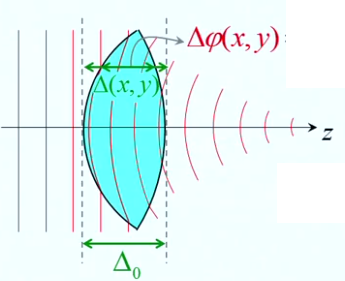
\includegraphics[scale=0.45]{ch3/image13.png}
	\captionof{figure}{ }
	\end{wrapfigure}		
	Dès lors, la phase accumulé dans la lentille vaudra simplement $\Delta \varphi(x,y) = k\Delta (x,y)$. 
	Comme on travaille sur la phase, il faut la définir pour une valeur de $z$ donnée (passage du plan 
	d'entrée au 	plan de sortie). Il faudra alors considérer la passage dans l'air, sans diffraction :
	\begin{equation}
	\Delta \varphi(x,y) = k\Delta (x,y) + k_0[\Delta_0-\Delta(x,y)]
	\end{equation}
	Il s'agit du déphasage introduit par la lentille en un point $(x,y)$ du plan transverse. Or, 
	$\Delta(x,y)$ est connu : à partir du champ dans le plan d'entrée $a(x,y)$ on pourra connaître le 
	champ $a'(x,y)$	dans le plan de sortie 
	\begin{equation}
	a'(x,y) = a(x,y)\underbrace{e^{i\Delta\varphi(x,y)}}_{T(x,y)}
	\end{equation}
	Le facteur de phase représente la phase accumulée du plan d'entrée au plan de sortie, y compris les 
	passages dans l'air. Attention, si la fonction de transfert ne contient que ceci, cela signifie que 
	que toute variation de l'amplitude du champ est négligée : l’absorption et les réflexions dans le 
	diélectrique sont négligées. Ceci définit la fonction de transfert $T(x,y)$.\\
	
	On peut écrire, en distribuant : $\Delta\varphi(x,y) = k_0\Delta_0 + (k-k_0)\Delta(x,y)$. Comme 
	$k=k_0n$, l'expression devient
	\begin{equation}
	\Delta\varphi(x,y) = k_0\left[\Delta_0+(n-1)\Delta(x,y)\right]
	\end{equation}
	En substituant l'expression de $\Delta(x,y)$ et après simplifications
	\begin{equation}
	\Delta \varphi(x,y) = k_0\left[n\Delta_0-(n-1)\dfrac{x^2+y^2}{2}\left(\dfrac{1}{R_1}+\dfrac{1}{R_2}\right)
	\right]
	\end{equation}
	Introduisons un nouveau paramètre
	\begin{equation}
	\frac{1}{f} \equiv (n-1)\left(\dfrac{1}{R_1}+\dfrac{1}{R_2}\right)
	\end{equation}
	afin d'écrire
	\begin{equation}
	\Delta\varphi(x,y) = k_0\left[n\Delta_0 - \dfrac{x^2+y^2}{2f}\right]
	\end{equation}
	Notre fonction de transfert devient alors
	\begin{equation}
	T(x,y) = e^{ik_0 n\Delta_0}\ e^{-i\frac{k_0}{2f}(x^2+y^2)}
	\end{equation}
	Le premier terme, de phase constante, revient à changer l'origine : on n'en tiendra pas compte ici (pas 
	d'interprétation physique si l'on n'étudie pas la dynamique de passage dans la lentille).
	En effet,
	
	\begin{equation}
	b(x,y)= a(x,y) e^{-i\omega_0 t} \Rightarrow b(x,y) = a(x,y) e^{-i\dfrac{k}{2f}(x^2+y^2)} \underbrace{e^{ik_0\Delta_0 n -i\omega_0t}}_{e^{-i\omega_0\left[t-\dfrac{k_0\Delta_0 n}{\omega_0}\right]}}
	\end{equation}
	
	On ne garde 
	que le terme de phase quadratique, ce qui est normal vu notre approximation parabolique. 
	\begin{equation}
	T(x,y) =\DS e^{\DS -i\frac{k_0}{2f}(x^2+y^2)}
	\end{equation}
	On verra que $f$ n'est autre que la \textit{distance focale} de la lentille (qui ne contient que l'indice de 
	réfraction et les rayons de courbures).

\newpage
\section{Fonction de transfert : interprétation}	
	\begin{wrapfigure}[10]{l}{7.4cm}
	\vspace{-5mm}
	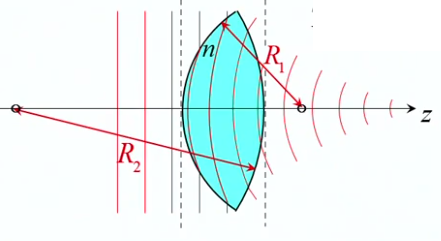
\includegraphics[scale=0.45]{ch3/image14.png}
	\captionof{figure}{ }
	\end{wrapfigure}		
Il est maintenant temps de faire l'interprétation physique de cette fonction. Le paramètre $f$ est défini 
par 
\begin{equation}
\frac{1}{f} \equiv (n-1)\left(\dfrac{1}{R_1}+\dfrac{1}{R_2}\right)
\end{equation}
L'indice de réfraction contient toute l'information du diélectrique, il est donc logique de le voir 
apparaître ici. On trouve également des paramètres géométriques.  Dans l'approximation des lentilles 
minces ($\Delta_0\ll R_1,R_2$ afin de négliger la diffraction entre le plan d'entrée et de sortie), nous 
avions obtenu
\begin{equation}
a'(x,y) = a(x,y)e^{-i\dfrac{k_0}{2f}(x^2+y^2)}
\end{equation}
Le terme de phase constant représentant la propagation dans la lentille a été négligé, celui-ci ne 
représentait qu'une modification de l'origine. \\

Dans le cadre de la description des lentilles minces, une lentille a une épaisseur dite "nulle" : on 
passe du plan $z=0^-$ au plan $z=0^+$. Cela permet de justifier le fait que l'on a omis le facteur de 
phase constante. \\

	\begin{wrapfigure}[12]{l}{8.4cm}
	\vspace{-5mm}
	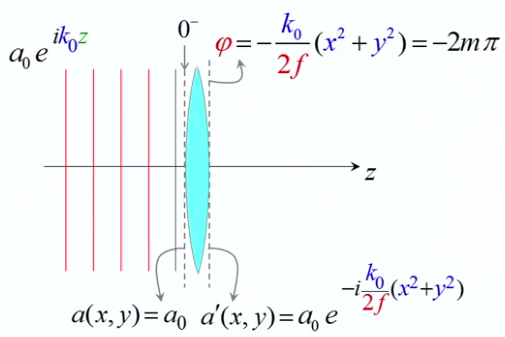
\includegraphics[scale=0.45]{ch3/image15.png}
	\captionof{figure}{ }
	\end{wrapfigure}		
Ce rappel étant fait, passons à l'interprétation. Considérons l'incidence d'une onde plane se propageant 
parallèlement à l'axe $z$ : une onde plane étant caractérisée par $a_0e^{ikz}$, évaluée en $z=0^-$ cela 
donne $a(x,y)=a_0$ comme suggérer ci-dessous :
\begin{equation}
a(x,y) = a_0 a'(x,y) = a_0e^{-i\dfrac{k_0}{2f}(x^2+y^2)}
\end{equation}
La distribution de phase dans le plan de sortie est donnée par la phase de la fonction de transfert. 
Étudions-la, que représente-t-elle ? Recherchons des "fronts d'onde", c'est-à-dire les lieux de phases 
constantes valant un multiple de $2\pi$ les lieux des points sur lequel le champ est maximum

	\begin{wrapfigure}[12]{r}{4cm}
	\vspace{-5mm}
	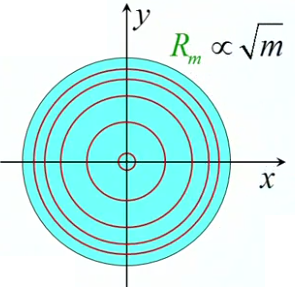
\includegraphics[scale=0.35]{ch3/image16.png}
	\captionof{figure}{ }
	\end{wrapfigure}	
\begin{equation}
\varphi = -\dfrac{k_0}{2f}\underbrace{(x^2+y^2)}_{R_m^2} = -2m\pi
\end{equation}

Le signe négatif est là pour la simplification. Représentons ce lieu des points dans le plan transverse, 
il s'agira bien entendu de cercles dont le rayon $R_m\propto \sqrt{m}$. On obtient ainsi l'interception
des fronts d'onde dans le plan de sortie.

\newpage
	\begin{wrapfigure}[8]{l}{4cm}
	%\vspace{-5mm}
	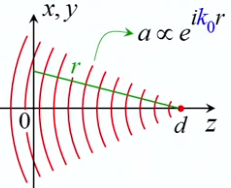
\includegraphics[scale=0.35]{ch3/image17.png}
	\captionof{figure}{ }
	\end{wrapfigure}	
Regardons maintenant ce que représente l'onde obtenue dans l'interception du plan de sortie. Pour se faire 
comparons la distribution de phase dans le plan $z=0^+$ à la distribution de phase d'une onde sphérique 
générée à un point $d$ de l'axe de la lentille. Dans le schéma ci-contre, $r$ est représenté jusqu'au plan 
de la lentille par facilité (et parce qu'on s'intéresse au plan de la lentille). Par Pythagore
\begin{equation}
r = \sqrt{d^2+x^2+y^2} \approx d + \dfrac{1}{2d}\left(x^2+y^2\right)
\end{equation}
La distribution de phase du champ de l'onde sphérique de l'onde dans le plan $z=0$ est alors donnée par
\begin{equation}
(x,y;0) \propto e^{ik_0d}\ e^{i\dfrac{k_0}{2d}(x^2+y^2)}
\end{equation}
Ceci ressemble à la distribution de phase obtenue à la sortie de la lentille. On peut également négliger 
le terme de phase constante. Une différence notable avec la sortie de la lentille est une différence de 
signe. Pour le comprendre, exprimons le champ avec sa dépendance temporelle
\begin{equation}
E(x,y,z,t) \propto e^{i(k_0r-\omega t)}
\end{equation}

	\begin{wrapfigure}[8]{r}{3.5cm}
	\vspace{-5mm}
	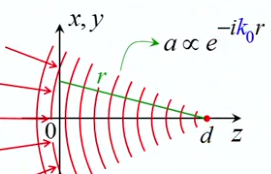
\includegraphics[scale=0.35]{ch3/image18.png}
	\captionof{figure}{ }
	\end{wrapfigure}
Les lieux de phases constantes en laissant filer le temps sont $\varphi = k_0 r-\omega t = c^{te}$. Lorsque 
le temps augmente, pour rester sur un front d'onde, il faut nécessairement que $r$ augmente pour compenser 
le signe négatif. Il s'agit d'une onde onde dont les rayons de courbure (le rayon $r$) augmente : onde 
sphérique divergente. En remplaçant un signe négatif dans notre onde sphérique l'onde sera bien convergente 
vers le \textit{foyer}. En effet, $\varphi = k_0 r+\omega t = c^{te}$, 
lorsque $t$ augmente, $r$ doit nécessairement diminuer \\

L'interprétation de la distribution de phase dans le plan de sortie n'est rien d'autre que la distribution 
de phase d'une onde convergente qui se focalise à la distance $f$ (si on remplace $d$ par $f$) 
la \textit{distance focale} de la lentille.\\

Une onde plane incidente sur la lentille donne une onde convergente au point focal $f$. Pour faire les 
choses plus rigoureusement, on peut appliquer la théorie de la diffraction pour montrer que la distribution 
de phase est bien celle d'une onde sphérique convergente. Prenons la formule de diffraction de Fresnel
\begin{equation}
a'(x,y,f) = \dfrac{k}{z}\iint a'(x',y';0^+) e^{i\frac{k}{2f}(x-x')^2}e^{i\frac{k}{2f}(y-y')^2}\ dx'dy'\ e^{ikf}
\end{equation}

	\begin{wrapfigure}[8]{l}{5.5cm}
	\vspace{-5mm}
	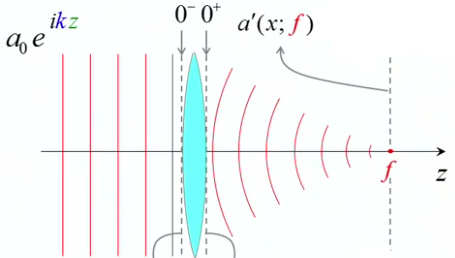
\includegraphics[scale=0.35]{ch3/image19.png}
	\captionof{figure}{ }
	\end{wrapfigure}
Il faut maintenant substituer l'expression de $a(x,y)$\footnote{Dans cette expression $k_0\rightarrow k$ car 
dans la théorie de Fresnel on travaillait déjà avec $k_0$ mais noté $k$.}. Pour simplifier, nous allons 
travailler à une seule dimension transverse
\begin{equation}
a'(x,f) = \sqrt{\dfrac{k}{f}}\int a'(x')e^{i\frac{k}{2f}(x-x')^2}\ dx'\ e^{ikf}
\end{equation}
La diffraction de ce champ jusqu'au point $f$ sera donné par application de la formule de Fresnel, ici à 
une dimension. 


\newpage
En substituant l'expression de $x'(x')$ 
\begin{equation}
a'(x,f) = \sqrt{\dfrac{k}{f}}\ a_0\int e^{\DS-i\frac{k}{2f}x^{'2}}\ e^{\DS i\frac{k}{2f}(x-x')^2}\ dx'\ e^{ikf}
\end{equation}
En effectuant le carré, l'expression se simplifie : le terme quadratique de phase en $x^{'2}$ se simplifie.
\begin{equation}
a'(x,f) = \sqrt{\dfrac{k}{f}}\ a_0\ e^{i\frac{k}{2f}x^2}\underbrace{\int  e^{\DS -i\frac{k}{f}xx'}\ dx}_{
\propto\ a_0\delta(x)}'\ e^{ikf}
\end{equation}
L'intégrale du facteur linéaire en $x'$ intégrée en $x'$ ne vaut zéro tant que le facteur avant le $x'$ 
n'est pas nul\footnote{?}, la seule valeur qui va en ressortir sera lorsque $x=0$. A la grosse louche, 
en deux dimension
\begin{equation}
a'(x,y;f) \propto\ a_0\delta(x,y)
\end{equation}
Le résultat de l'intégrale de Fresnel au point $f$ étant une delta de Dirac, l'onde se focalise au point 
$f$ : il s'agit bien d'une onde sphérique convergente.\\

	\begin{wrapfigure}[8]{l}{5.5cm}
	\vspace{-5mm}
	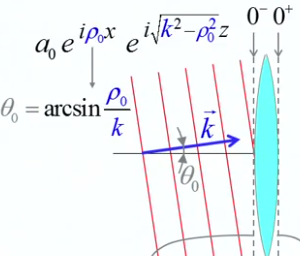
\includegraphics[scale=0.35]{ch3/image20.png}
	\captionof{figure}{ }
	\end{wrapfigure}
Généralisons en considérant une onde d'incidence oblique à l'aide du vecteur d'onde $\vec{k}$. Comme 
précédemment, le choix de $\rho_0$ fixe l'angle $\theta_0$. Dans le plan d'entrée de la lentille, on 
trouve
\begin{equation}
a(x,y) = a_0\ e^{i\rho_0x}
\end{equation} 
Ce qui multiplié par la fonction de transfert donne
\begin{equation}
a'(x,y) = a_0\ e^{i\rho_0x}\ e^{-i\dfrac{k}{2f}(x^2+y^2)}
\end{equation}
Étudions maintenant la diffraction de Fresnel (toujours à une dimension). En remplaçant le champ dans 
le plan incident et après simplification (comme précédemment) :
\begin{equation}
a'(x,f) = \sqrt{\frac{k}{f}}\ a_0\ e^{i\frac{k}{2f}x^2} \underbrace{\int e^{i\rho_0x'}\ e^{-i\frac{k}{f}xx'}\ dx'}_{
\propto\ a_0\delta(x-\frac{\rho_0f}{k} )} 
e^{ikf}
\end{equation}
Le résultat sera analogue au précédent : le champ transmis donne un pic d'intensité dans le plan focal de 
la lentille.
\begin{equation}
a'(x,y;f) \propto a_0\left(x-\dfrac{\rho_0f}{k},y\right)
\end{equation}

	\begin{wrapfigure}[8]{r}{7.5cm}
	\vspace{-5mm}
	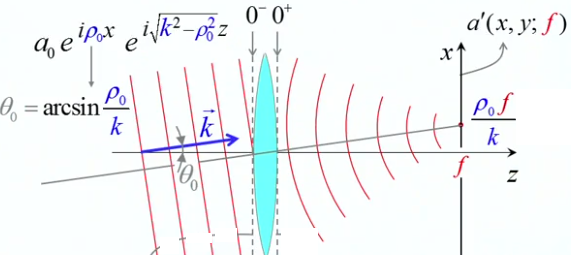
\includegraphics[scale=0.4]{ch3/image21.png}
	\captionof{figure}{ }
	\end{wrapfigure}
Le foyer ne se trouve plus sur l'axe focal mais bien dans le même plan que celui-ci : il s'agit du 
\textit{plan focal} et on parle de \textit{foyer secondaire}. A quoi correspond cette hauteur du 
point focal ? Sachant que $\rho_0/k = \sin\theta$ :
\begin{equation}
\dfrac{\rho_0f}{k} = f\sin\theta \approx f\theta_0 \approx f\tan\theta
\end{equation}
Ceci montre que la hauteur obtenue est la hauteur obtenue par la projection d'un rayon parallèle à $\vec{k}$, 
passant par le centre de la lentille, dans le plan focal. Cela permet d'établir la \textit{théorie des rayons}.\\

	\begin{wrapfigure}[9]{l}{5.5cm}
	\vspace{-5mm}
	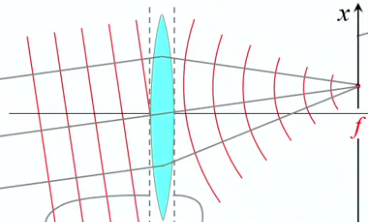
\includegraphics[scale=0.4]{ch3/image23.png}
	\captionof{figure}{ }
	\end{wrapfigure}
Les rayons sont ainsi des lignes partout perpendiculaires aux fronts d'onde (qui ne sera pas toujours 
droite). Ainsi, deux rayons parallèles devant la lentille se croisent dans le plan focal, au \textit{foyer secondaire}. 
Par réciprocité (revenons dans le temps), deux rayons émanant du point focal sont parallèles de l'autre côté de la 
lentille : on retrouve les règles de l'optique géométrique, tout est décrit dans la fonction de transfert.\\

Passons maintenant à l'interprétation physique de la fonction de transfert. Considérons n'importe quelle 
onde incidente sur la lentille. Solution des équations de Maxwell, on peut toujours la représenter comme
une somme d'onde planes (monochromatique, sans dépendance temporelle)
\begin{equation}
a(x;z) = \int A(\rho)e^{i\rho x}e^{i\sqrt{k^2-\rho^2}z}\ d\rho
\end{equation}
Tout onde peut être exprimée comme une somme d'onde plane, d'où l'importance de la précédente analyse : 
le principe de superposition va nous être précieux. Évalué dans le plan d'entrée de la lentille 
\begin{equation}
a(x;0) = \int A(\rho)e^{i\rho x}\ d\rho
\end{equation}
Commençons par regarder un terme de cette somme. Si l'on regarde le cas précédemment traité, nous 
avions $a(x) = a_0 e^{i\rho_0x}$. La différence est le changement suivant : $a_0\rightarrow A(\rho)d\rho$.
En substituant dans l'expression précédemment obtenue pour $a'(x;f)$ :
\begin{equation}
a'(x;f) \propto\ A(\rho)\delta\left(x-\frac{\rho f}{k}\right)\ d\rho
\end{equation}

	\begin{wrapfigure}[10]{r}{5cm}
	\vspace{-5mm}
	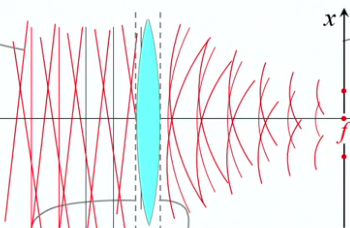
\includegraphics[scale=0.4]{ch3/image22.png}
	\captionof{figure}{ }
	\end{wrapfigure}
Ce qui a été fait pour une onde plane est vrai pour toute onde plane et par la principe de superposition, 
nous pouvons sommer le résultat. 

\begin{equation}
a'(x;f) \propto\ \int A(\rho)\delta\left(x-\frac{\rho f}{k}\right)\ d\rho
\end{equation}
On obtient le spectre multiplié par une delta de Dirac. En appliquant la Dirac
\begin{equation}
a'(x;f) \propto A\left(\dfrac{kx}{f}\right)
\end{equation}
La distribution à la sortie est donnée par le spectre du champ incident pour la variable $\rho$ devenue 
$kx/f$, la variable de Fourier est devenue une variable spatiale.\\

Pour l'interpréter, imaginons que l'on place un plan transparent sur le plan optique. Si l'on regarde 
le point $x_0$, celui-ci est le point focale d'une onde sphérique : on "sélectionne" une onde plane 
d'angle $\theta_0 = x_0/f$. On observe ainsi l'amplitude d'une onde d'angle $x_0/f$. Or, chaque valeur 
de $\theta$ correspond à une valeur de $\rho \longrightarrow \rho_0 = k\dfrac{x_0}{f}$.\\

Tout est cohérent, le $x_0$ sélectionne un $\rho_0$. A une hauteur $x$ donnée on retrouve bien 
l'amplitude du champ conditionnée à la hauteur où l'on regarde. 


\newpage
\section{Les lentilles et transformée de Fourier}
Une lentille effectue la TF du champ qui lui est incident, le but est d'ici de voir ça de façon 
plus rigoureuse. Avant ça, interprétons physiquement notre dernier résultat, à savoir
%	\begin{wrapfigure}[12]{l}{9.7cm}
%	\vspace{-5mm}
%	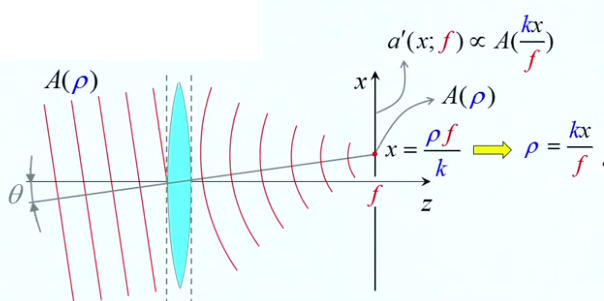
\includegraphics[scale=0.45]{ch3/image24.png}
%	\captionof{figure}{ }
%	\end{wrapfigure}		
\begin{equation}
a'(x,f)\propto A\left(\frac{kx}{f}\right)
\end{equation}
Pourquoi une lentille effectue-t-elle dans son plan focal la transformée de Fourier du plan qui 
lui est incident ? On peut voir le champ incident comme une superposition d'onde plane
\begin{equation}
a(x;z) = \int A(\rho)e^{i\rho x}e^{i\sqrt{k^2-\rho^2}z}\ d\rho
\end{equation}
où l'on reconnaît le spectre en $z=0$ (le propagateur tombe).  Considérons une des composantes de 
cette somme, à savoir une onde plane pour une valeur $\rho$. Celle-ci se transforme en onde 
sphérique pour se focaliser dans le plan focal en un foyer (ici secondaire) $x=\frac{\rho f}{k}$. 
On le sait car on peut dire que cette valeur de $x$ sélectionne une onde plane avec une certaine 
valeur de $\rho$, c'est-à-dire un angle $\theta$. L'amplitude de la delta de Dirac au point de 
focalisation vaut alors $A(\rho)$. Le $\rho$ dans $A(\rho)$ doit être traduit en terme de distribution 
dans le plan d'observation : il faut le décrire par rapport à la variable $x$. En isolant $\rho$ 
dans l'expression de $x$ on trouve
\begin{equation}
\rho = \dfrac{kx}{f}
\end{equation}
où $x/f = \tan\theta \approx \theta$. En ré-écrivant $A(\rho)$, on a bien le spectre en $kx/f$ :
\begin{equation}
A(\rho)\qquad\Longrightarrow\qquad A\left(\frac{kx}{f}\right)
\end{equation}
Nous ne connaissons qu'un facteur de proportionnalité, on peut s'attendre à trouver une distorsion 
de phase : le champ obtenu dans le plan focal contient la transformée de Fourier mais pas seulement.\\


	\begin{wrapfigure}[10]{l}{6.5cm}
	\vspace{-5mm}
	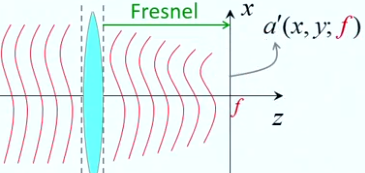
\includegraphics[scale=0.5]{ch3/image25.png}
	\captionof{figure}{ }
	\end{wrapfigure}		
Considérons un champ incident quelconque et étudions le champ dans un plan. Nous connaissons 
la fonction de transfert de la lentille
\begin{equation}
T(x,y) = e^{-i\frac{k}{2f}(x^2+y^2)}
\end{equation}
mais également la diffraction de Fresnel. La fonction de transfert nous informera ce qui se passe 
entre le plan entrant $a(x,y;0^-)$ et sortant $a(x,y;0^+)$ :
\begin{equation}
a(x,y;0^+) = a(x,y;0^-)e^{-i\frac{k}{2f}(x^2+y^2)}
\end{equation}
Fresnel nous donne la propagation du champ entre $z=0^+$ jusqu'au plan $z=f$ avec sa fameuse formule 
de diffraction:
\begin{equation}
a(x,y;z) = \frac{k}{z}\int a(x',y';0)\ e^{i\dfrac{k}{2z}(x-x')^2}\
 e^{i\dfrac{k}{2z}(y-y')^2}\ dx'dy'\  e^{ikz}
\end{equation}
Nous obtenons alors
\begin{equation}
a(x,y;f) = \dfrac{k}{f}\int a(x,y;0^-)e^{-i\frac{k}{2f}(x^{'2}+y^{'2})}\ e^{i\dfrac{k}{2z}(x-x')^2}\
 e^{i\dfrac{k}{2z}(y-y')^2}\ dx'dy'\  e^{ikf}
\end{equation}
Sachant que $(x-x')^2 = (x^2-2xx'+x^{'2})$ et de même pour le terme en $y$, on peut finalement 
obtenir (le facteur en $x^2$ et $y^2$ peuvent sortir de l'intégrale)
\begin{equation}
a(x,y;f) = \dfrac{k}{f}e^{i\frac{k}{2f}(x^2+y^2)}\int a(x,y;0^-)e^{-i\frac{k}{f}xx'}\ e^{-i\frac{k}{f}yy'}\  
dx'dy'\  e^{ikf}
\end{equation}
Il s'agit d'une intégrale avec des facteurs de phases linéaires. On peut faire apparaître la définition de 
la transformée de Fourier d'un champ
\begin{equation}
A(\rho, \sigma) = \int a(x',y',0)e^{-i\rho x'}e^{-i\sigma x'}\ dx'\ dy'
\end{equation}
Il nous suffit d'identifier : $\rho = kx/f$ et $\sigma = ky/f$.
\begin{equation}
a(x,y;f) = \dfrac{k}{f}e^{ikf} e^{i\frac{k}{2f}(x^2+y^2)}A\left(\frac{kx}{f},\frac{ky}{f}\right)  
\end{equation}
On voit que la lentille ne donne pas strictement une transformée de Fourier : celle-ci est multipliée 
par un facteur de phase quadratique.  Le résultat est quasi-identique à celui de Fraunhofer à une 
différence près : la distance de $z$ est finie et pas juste "suffisamment grande" comme c'était le cas 
pour Fraunhofer (nous avons ici juste fait l'approximation paraxiale).
\begin{equation}
a(x,y;z) = \dfrac{k}{z} e^{ikz} e^{i\dfrac{k}{2}(x^2+y^2)}\ A\left(\frac{kx}{z},\frac{ky}{z}\right)
\end{equation}
Nous allons faire l'analogie avec Fraunhofer. Si l'on n'observe que l'intensité (module carré du 
champ), la densité spectrale, celle-ci correspond bien à "seulement la transformée de Fourier". Comment 
interpréter ce facteur de phase additionnel ? \\

	\begin{wrapfigure}[8]{r}{5cm}
	\vspace{-8mm}
	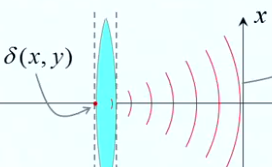
\includegraphics[scale=0.5]{ch3/image26.png}
	\captionof{figure}{ }
	\end{wrapfigure}		
Considérons comme champ incident une delta de Dirac centrée à l'origine, 
comme on néglige la diffraction dans la lentille, on aura une onde sphérique à la sortie de lentille :
ceci devrait générer une onde sphérique (de Huygens dans le cadre de Fraunhofer).
Ceci est totalement logique, le spectre de la 
fonction de Dirac est une constante :
\begin{equation}
A\left(\frac{kx}{f},\frac{ky}{f}\right)=1
\end{equation}
Dès lors
\begin{equation}
a(x,y;f) = \DS \dfrac{k}{f}e^{ikf} e^{i\frac{k}{2f}(x^2+y^2)}
\end{equation}

	\begin{wrapfigure}[9]{l}{5cm}
	\vspace{-12mm}
	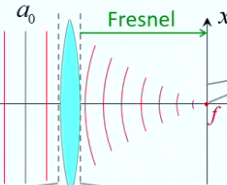
\includegraphics[scale=0.5]{ch3/image27.png}
	\captionof{figure}{ }
	\end{wrapfigure}	
Considérons cette fois un champ constant incident sur notre lentille. Celui-ci à une amplitude $a_0$ et 
une incidence nulle. Le spectre d'une constante étant une delta de Dirac, on obtient le résultat attendu
\begin{equation}
a'(x,y;z) = \frac{k}{f}e^{ikf}a_0\delta(x,y)
\end{equation}
Généralisons à toute distance  : on ne s'intéressant qu'au plan d'entrée, considérons maintenant une 
distance $d_0$ du plan d'entrée et on s'intéresse au champ dans le plan focal. Pour se faire, rappelons 
que le spectre $A(kx/f,ky/f)$ provient de la transformée de Fourier du champ en $z=0^-$. Comment faire 
apparaître le champ en $-d_0$ ? Utilisons Fresnel, mais de façon intelligente : le résultat étant donné 
en fonction du spectre en $z=0^-$, nous n'allons pas exprimer le spectre dans le domaine spatial (soit 
le point de départ de sa théorie) :
\begin{equation}
a(x,y;z) = \iint A(\rho,\sigma;0)e^{i\rho x}e^{i\sigma y} e^{-i\frac{\rho^2}{2k}z}
e^{-i\frac{\sigma^2}{2k}z}\ d\rho d\sigma\ e^{ikz}
\end{equation}

	\begin{wrapfigure}[10]{r}{8cm}
	\vspace{-2mm}
	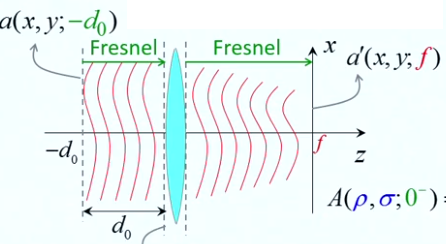
\includegraphics[scale=0.5]{ch3/image28.png}
	\captionof{figure}{ }
	\end{wrapfigure}	
Ceci dit qu'un champ peut être décomposé en onde plane où le propagateur s'est vu approximer par l'
approximation paraxiale. Ceci nous donne le champ en $z$ à partir du spectre en 0. Le propagateur 
apporte bien la diffraction. On y voit un nouveau spectre qui n'est plus $A(\rho,\sigma;0)$ mais
\begin{equation}
A(\rho,\sigma;z) = A(\rho,\sigma;0)e^{-i\frac{\rho^2}{2k}z}e^{-i\frac{\sigma^2}{2k}z} e^{ikz}
\end{equation}
Il s'agit de la \textit{propagation du spectre} : la multiplication du spectre par son propagateur 
donne le spectre à un autre endroit. Ceci montre donc comment se propage un spectre sur une distance 
$z$ (de 0 en $z$).  On peut utiliser cette expression pour une propagation sur une distance $d_0$ 
\begin{equation}
A(\rho,\sigma;0) = A(\rho,\sigma;-d_0)e^{i\frac{\rho^2}{2k}d_0-i\frac{\sigma^2}{2k}d_0} e^{ikd_0}
\end{equation}
En substituant $\rho$ et $\sigma$ :
\begin{equation}
A(\frac{kx}{f},\frac{ky}{f};0) = A(\frac{kx}{f},\frac{ky}{f};-d_0)e^{-\frac{i}{2k}\left(\frac{kx}{f}\right)^2d_0}e^{-
\frac{i}{2k}\left(\frac{ky}{f}\right)^2d_0} e^{ikd_0}
\end{equation}

	\begin{wrapfigure}[10]{l}{7cm}
	\vspace{-5mm}
	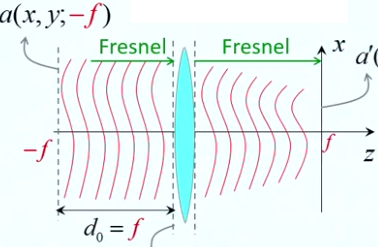
\includegraphics[scale=0.5]{ch3/image29.png}
	\captionof{figure}{ }
	\end{wrapfigure}
En simplifiant et en considérant une distance objet valant la distance focale $d_0=f$ :
\begin{equation}
A(\frac{kx}{f},\frac{ky}{f};0) = A(\frac{kx}{f},\frac{ky}{f};-f)e^{-\frac{k}{2f}x^2}e^{-\frac{k}{2f}y^2}
e^{ikf}
\end{equation}
En substituant ce résultat 
\begin{equation}
a(x,y;f) = \dfrac{k}{f}e^{ikf} e^{i\frac{k}{2f}(x^2+y^2)}A(\frac{kx}{f},\frac{ky}{f};-f)e^{-\frac{k}{2f}x^2}e^{-\frac{k}{2f}y^2}
e^{ikf}
\end{equation}
Les facteurs quadratiques se simplifie : il n'y a plus d'autres dépendances en $x,y$ que celles du 
spectre de l'onde
\begin{equation}
a(x,y;f) = \dfrac{k}{f}e^{2ikf} A\left(\frac{kx}{f},\frac{ky}{f};-f\right)
\end{equation}
Ceci montre que grâce à une lentille, on peut retrouver la transformée exacte d'un champ (on fait de 
l'optique qualitative, pas besoin des termes constant devant) si le champ est considéré à la distance 
focale $d_0=f$. 
\begin{equation}
a(x,y;f) \propto A\left(\frac{kx}{f},\frac{ky}{f};-f\right)
\end{equation}
Dans le plan focal image, nous aurons la transformée de Fourier \textbf{exacte} de ce champ pour un 
champ incident à $d_0=f$.







